\documentclass[a4paper,11pt]{article}
\usepackage[left=2.5cm, right=2.5cm, top=1.5cm, bottom=1.5cm]{geometry}
\usepackage{graphicx}
\usepackage{amssymb}
\usepackage{amsmath}
\usepackage{hyperref}
\usepackage{cleveref}
\usepackage{float}
\usepackage[table,xcdraw]{xcolor}
\usepackage{subcaption}

\hypersetup{ %color attributes of citation, link, etc.
    colorlinks=true,
    linkcolor=blue,
    filecolor=gray,
    urlcolor=blue,
    citecolor=blue,
}

\setlength{\parindent}{0pt}

\newcommand{\matlab}{\textsc{Matlab}} %very important and totally necessary addition
\newcommand{\parallelsum}{\mathbin{\!/\mkern-5mu/\!}}

\newcommand\Item[1][]{%
  \ifx\relax#1\relax  \item \else \item[#1] \fi
  \abovedisplayskip=0pt\abovedisplayshortskip=0pt~\vspace*{-\baselineskip}}

%'codify' text for snippets
\usepackage{xcolor}
\definecolor{codegray}{gray}{1}
\newcommand{\code}[1]{\colorbox{codegray}{\texttt{#1}}}


\graphicspath{ {./images/} }
           
\begin{document}
\title{\LARGE{\textbf{ECEN405 D-Class Amplifier}}\\ \large{\textit{`What a buck converter would say if it could talk'}}}
\author{Niels Clayton : 300437590\\
\textbf{Team Members:} Daniel Eisen \& Nickolai Wolfe}
\date{}
\maketitle

\begin{center}
    \vspace{-20pt}
    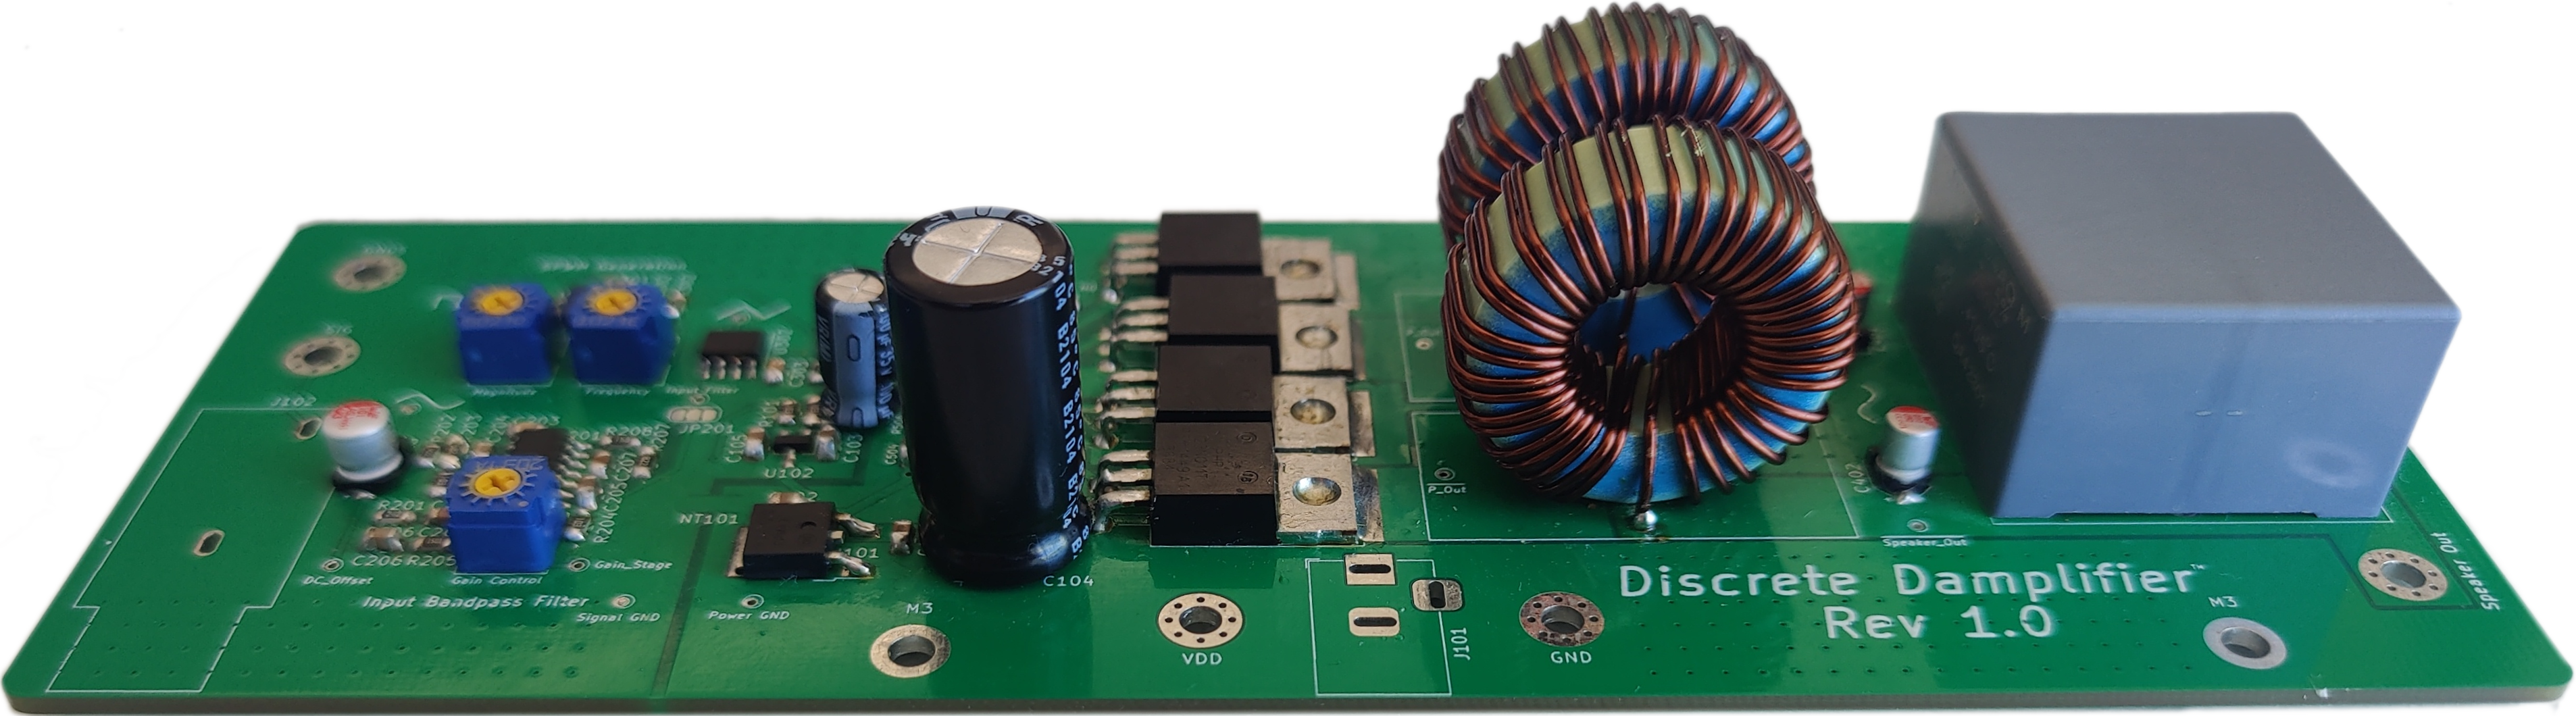
\includegraphics[width=0.9\textwidth]{design.png}
\end{center}

\section{Introduction}\label{S:intro}

Audio amplifiers facilitate the driving of high power speakers from small signal audio outputs. Common amplifier types for high fidelity audio are the class A and AB amplifier. These amplifiers provide high power outputs and very little distortion, with the limitation of low power efficiency. The efficiency losses in these topologies are due to the continuous operation of their amplifying elements (usually BJT's) within their saturation region, generating large continuous losses in the form of heat.

In contrast, the class D amplifier is a high efficiency power amplifier. These high efficiencies are achieved through the use of switching elements as amplifiers, allowing for no continuous power loss within the design. This topology can provide efficiencies of up to 90-95\%, with the limitation of greatly increased design complexity.\\

The purpose of this reports is to discuss the design and implementation of a class D amplifier for use in driving a sub-woofer speaker to given specifications outlined in \Cref{S:specs}. This project was completed in a group of three, where I have taken responsibility for the audio sampling and sinusoidal pulse width modulation (SPWM) generation designs. We have all contributed equally to the final PCB and schematic designs. 

\subsection{Specifications}\label{S:specs}

\begin{itemize}
    \item Supply 80W of power into a 4$\Omega$ load $\rightarrow P_{out} = 80W$ for $R_L = 4\Omega$.
    \item Have a 10Hz to 200Hz operating bandwidth.
    \item Have an input sensitivity of 1V for maximum output.
    \item Cost a maximum of \$50 per unit.
\end{itemize}

\section{Design}\label{S:design}

The operation of a class D amplifier can be broken down into discrete sections that are outlined in \Cref{F:block}. From this figure we see that the first section is the input audio signal filter, which acts to remove unwanted signal components from the input audio before amplification. In the next stage this filtered audio is sampled at high frequency using a triangle wave and a comparator to produce a high frequency SPWM carrier signal. Finally, this SPWM signal is then amplified to a high power output with a MOSFET before being low pass filtered again to remove the SPWM carrier frequency.

\begin{figure}[h!]
    \centering
    \frame{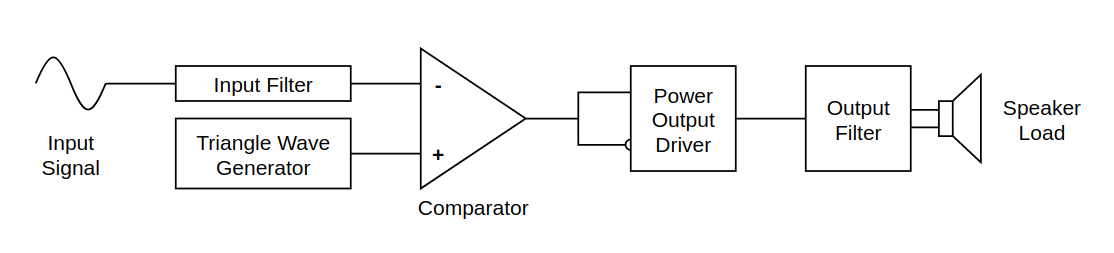
\includegraphics[width=0.8\textwidth]{block_diagram.png}}
    \caption{D-Class amplifier high level block diagram}
    \label{F:block}
\end{figure}

\subsection{High Level Design Decisions}

The high level design of this class D amplifier consisted of two decision, the selection of amplifier topology, and the selection of the input supply voltage level and supplies.\\

The exists two topologies for the design of class D amplifiers, half-bridge and full-bridge. The differentiating feature of these topologies is the configuration of their switching elements, with full-bridge requiring four MOSFETS and two gate drivers, while half-bridge requires two MOSFETS and a single gate driver. This has the affect of requiring the half-bridge topology to drive both the positive and negative portions of the output through a single MOSFET bridge, therefore requiring double the input voltage to achieve the same output power as the full-bridge topology. The half-bridge topology can also cause large fluctuations in the supply rail for the amplification, and therefore will often be accompanied by a feedback controller to account for these supply changes. Because of the design complications of the half-bridge topology, our design will implement the full-bridge class D amplifier.\\

For the selection of the designs power supply, it was decided that a single supply rail should be provided to the amplifier, with all other required voltage levels being generated internally. This was selected to provide a more cohesive and easy to operate final design. Based on this design, the required input voltage ($V_{DD}$) to achieve the specified output power of 80W has been calculated in the following equation to be 26V. This is then stepped down to both 12V and 5V internally though thee use of linear regulators. A 1000$\mu$F reservoir capacitor was also selected to reduce the strain on the input power supply from the high frequency high power switching elements.

$$ V_{DD} = \sqrt{2\cdot R_L \cdot P_{out}} = \sqrt{2\cdot 4 \cdot 80} = 25.29 \approx 26$$

In \Cref{F:design_schemtaic} we can see the finalised high-level schematic design of the amplifier. In this schematic the input supply stages can be found, as well as the high level design of the amplifier as discussed in \Cref{S:design}. 

\begin{figure}[h!]
    \centering
    \frame{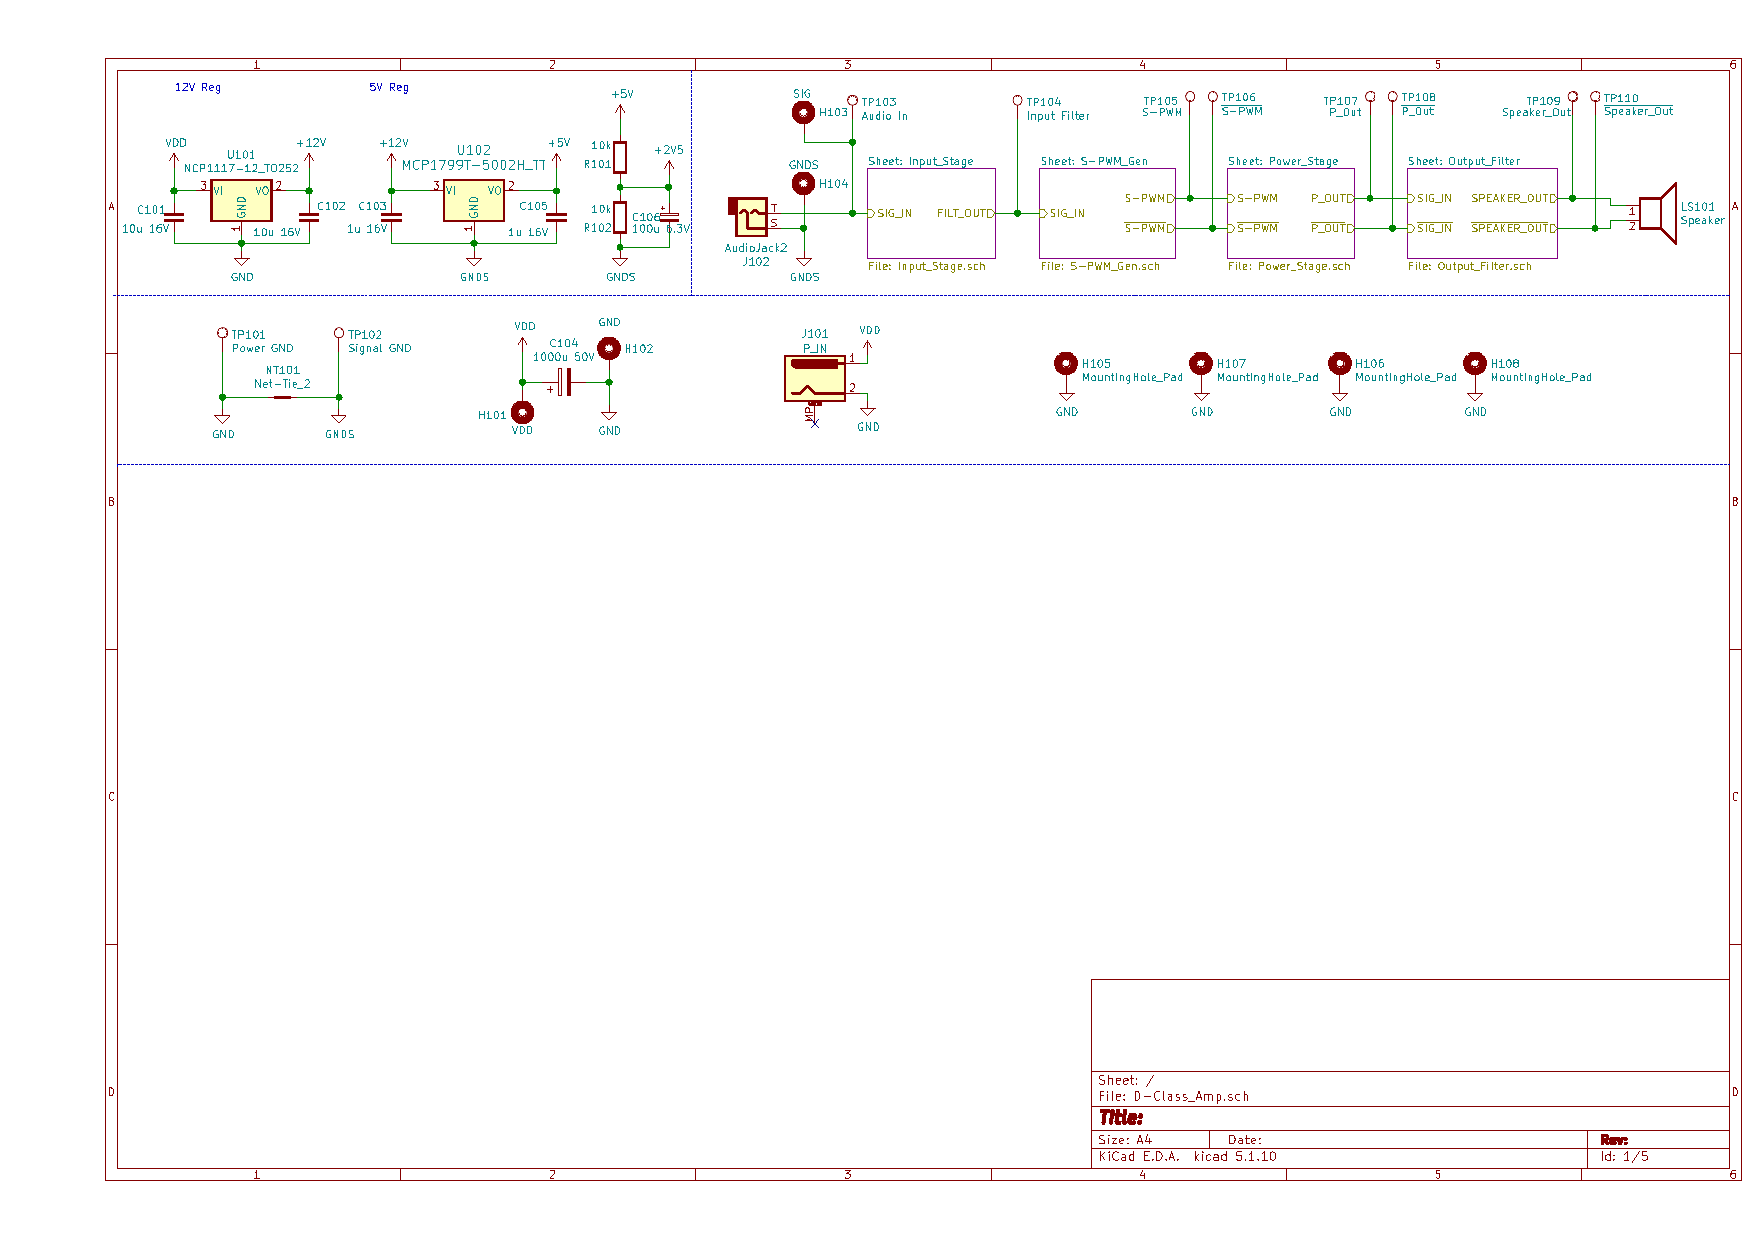
\includegraphics[page=1, trim={18mm 132mm 2mm 10mm},clip,width=0.85\textwidth]{pcb/schematic.pdf}}
    \caption{High level design schematic}
    \label{F:design_schemtaic}
\end{figure}

\subsection{Input Filter}

The design of the input filter was required to provide a signal passband of 10Hz to 200Hz, and function correctly for input signals of up to 1V amplitude, 2V$_{pk-pk}$ as specified in \Cref{S:specs}. The design of this section was undertaken by Nickolai Wolfe, and the finalised schematic of this can be seen in \Cref{F:input_filter_design}.


\begin{figure}[h!]
    \centering
    \frame{\includegraphics[page=2, trim={25mm 70mm 90mm 60mm},clip,width=0.85\textwidth]{pcb/schematic.pdf}}
    \caption{Input filtering schematic}
    \label{F:input_filter_design}
\end{figure}

This design consists of a forth order low pass active Butterworth filter with a cut-off frequency of 300Hz, and a second order high pass active Butterworth filter with a cut-off frequency of 10Hz. This provides 40dB per decade gain roll-off for inputs frequencies below 10Hz, as well as a 80dB per decade gain roll-off for inputs frequencies above 300Hz. It should also be noted that the placement of the low pass corner frequency at 300Hz ensures that there is a constant 0dB gain across the full specified bandwidth of the amplifier. \\

The output signal of the input filter has a DC bias of 2.5V imposed on it. This has been implemented to `mid-rail' the opamps utilised within this design, allowing them to function correctly from a single 5V DC supply.

This input stage also provides an amplifier gain stage to allow for tuning of the filter output amplitude.   

\subsection{Audio Sampling \& SPWM}

\begin{align*}
    f &= \frac{R_2}{4(R_1 \cdot R_2 \cdot C_1)} 
\end{align*}

\begin{figure}[h!]
    \centering
    \frame{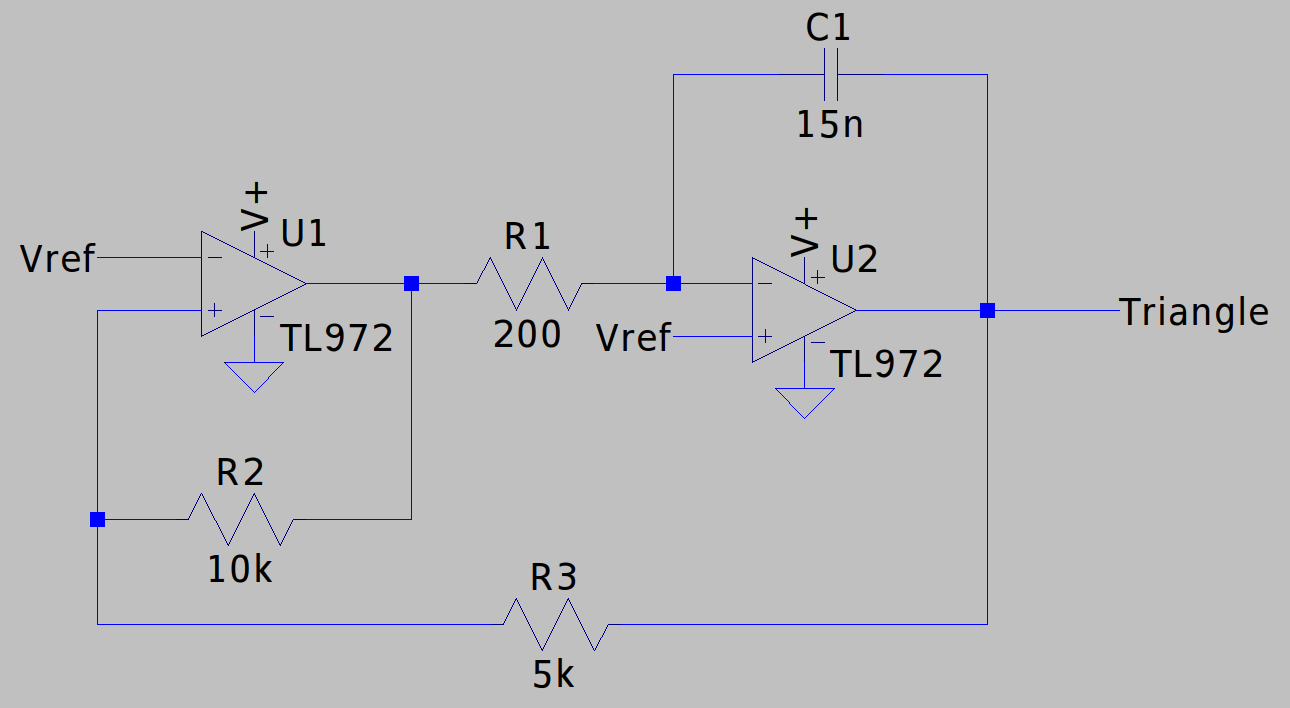
\includegraphics[width=0.5\textwidth]{spwm/circuit.png}}
    \caption{Triangle waveform generation circuit}
\end{figure}

\begin{figure}[h!]
    \centering
    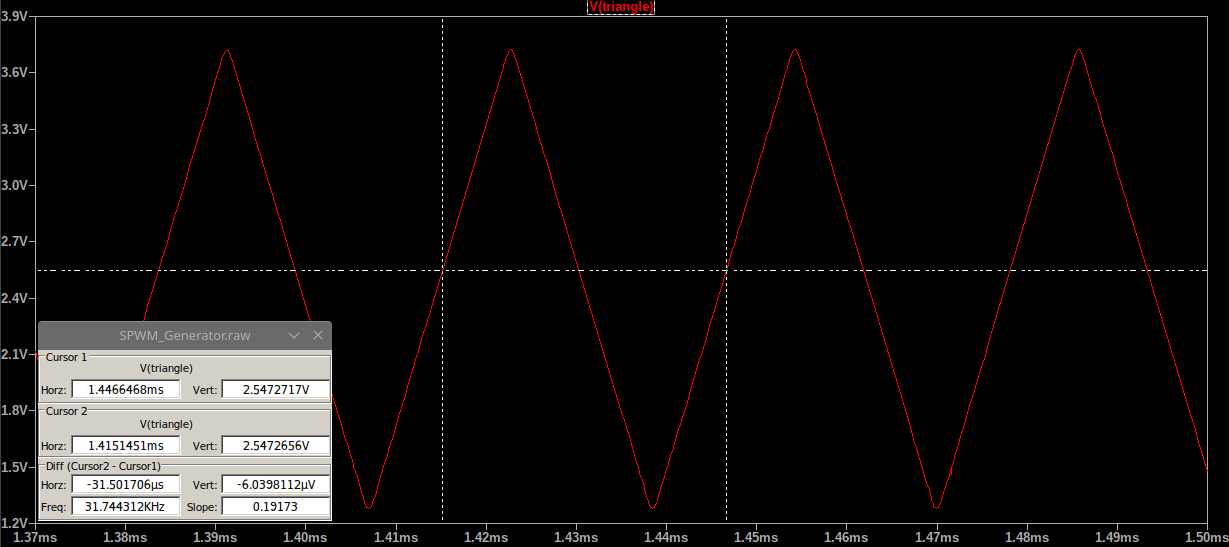
\includegraphics[width=0.8\textwidth]{simulation/triangle_wave.png}
    \caption{Simulation of the generated 32kHz triangle waveform}
\end{figure}


\begin{figure}[h!]
    \centering
    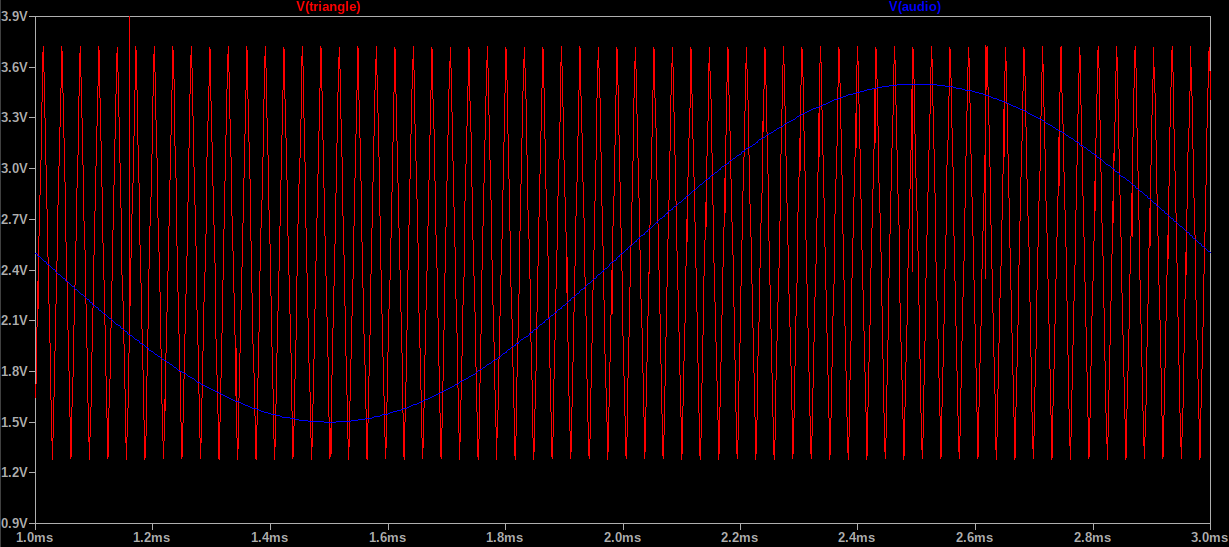
\includegraphics[width=0.8\textwidth]{simulation/sampling.png}
    \caption{Simulation of a 1V peak to peak input signal sampling}
\end{figure}


\begin{figure}[h!]
    \centering
    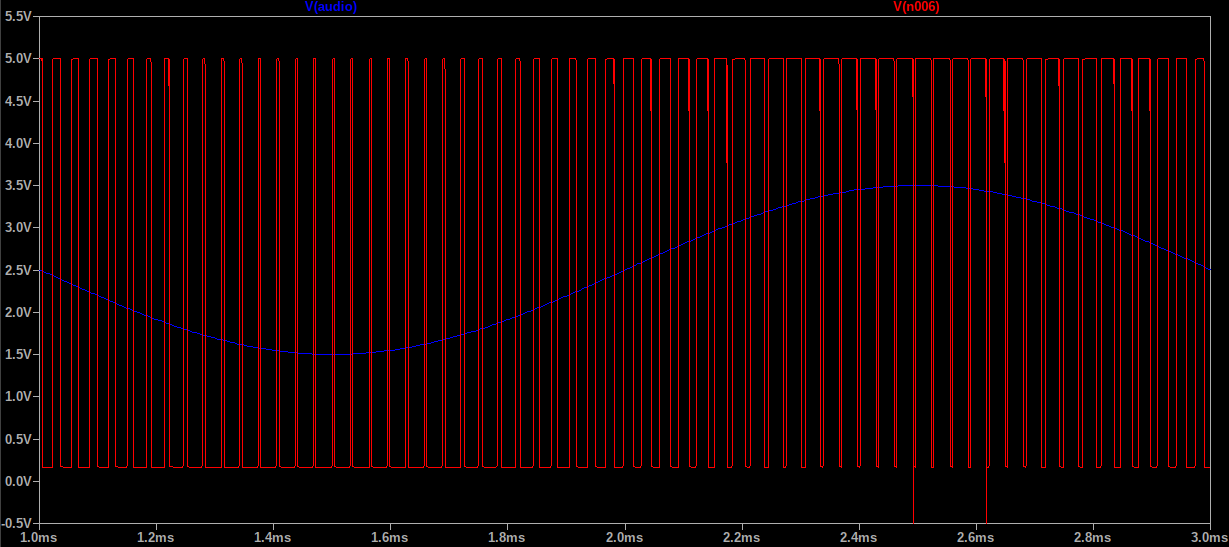
\includegraphics[width=0.8\textwidth]{simulation/spwm_out.png}
    \caption{Simulation of the SPWM comparator output}
\end{figure}

\begin{figure}[h!]
    \centering
    \frame{\includegraphics[page=3, trim={35mm 133.5mm 30mm 15mm},clip,width=0.85\textwidth]{pcb/schematic.pdf}}
    \caption{Sampling triangle wave \& SPWM generation schematic}
\end{figure}

\subsection{Power Stage \& Output Filter}

\begin{figure}[h!]
    \centering
    \frame{\includegraphics[page=5, trim={85mm 149mm 5mm 12mm},clip,width=0.85\textwidth]{pcb/schematic.pdf}}
    \caption{Gate driver schematic}
\end{figure}

\begin{figure}[h!]
    \centering
    \frame{\includegraphics[page=4, trim={115mm 97mm 105mm 75mm},clip,width=0.6\textwidth]{pcb/schematic.pdf}}
    \caption{Output filter schematic}
\end{figure}

\section{Implementation}

Here you should discuss the assembly of the amplifier and any problems you faced as a team building the amplifier.

Here, the individual components should also be characterised. For example: if you have a filter, what is the response and how does it compare to the calculated? If you have a triangle wave, how does it look? Is it doing what I should? Why? Why not? How do the inputs/outputs of your comparator look? How does the square wave on the gate of the MOSFETs look?

\subsection{PCB Design and Layout}

\begin{figure}[h!]
    \centering
    \begin{subfigure}{0.8\textwidth}
        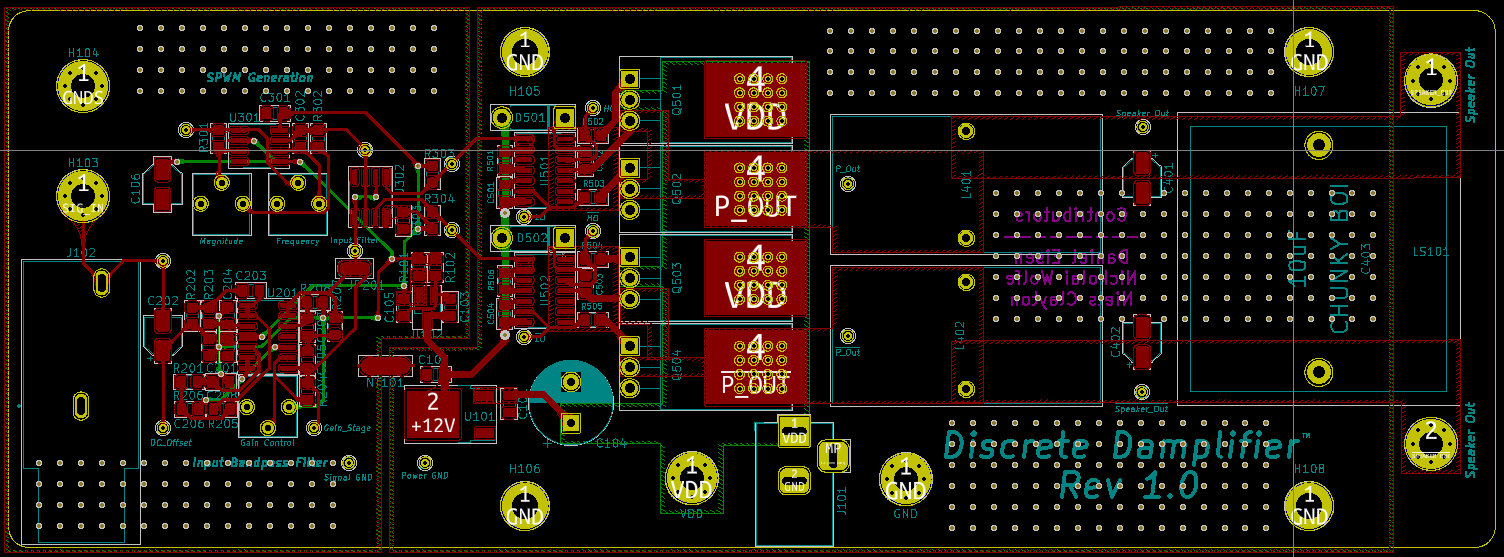
\includegraphics[width=\columnwidth]{pcb/traces.png}
        \subcaption{PCB Traces}
    \end{subfigure}
    \begin{subfigure}{0.8\textwidth}
        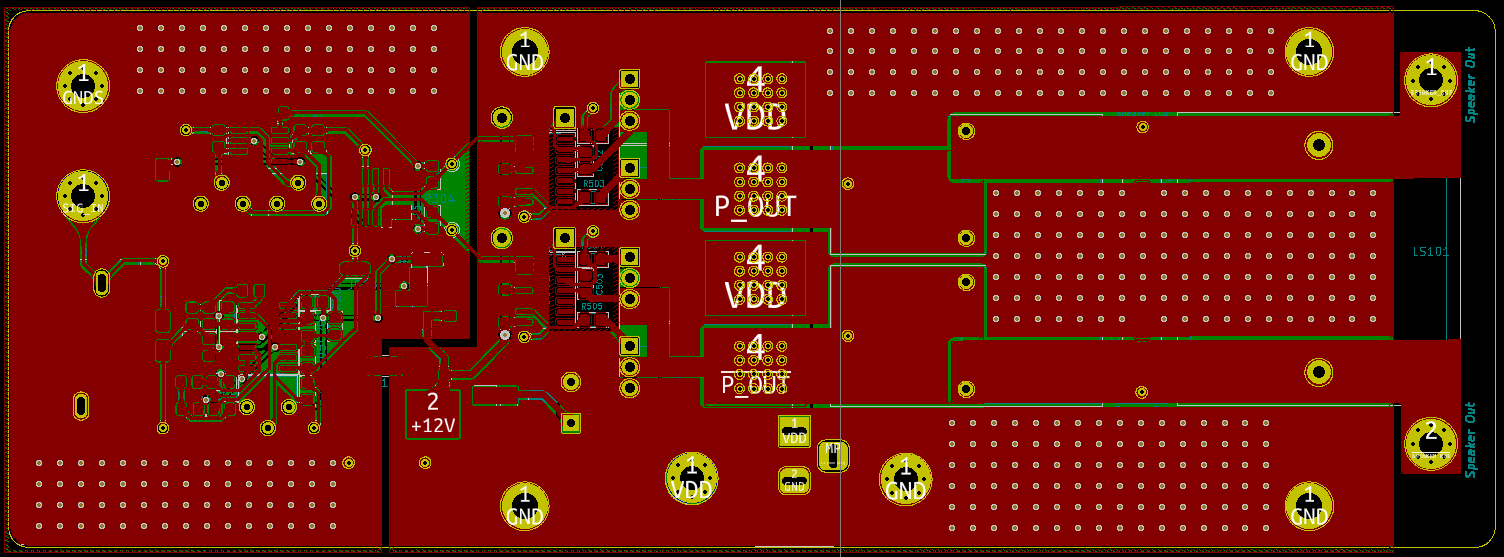
\includegraphics[width=\columnwidth]{pcb/top_layer.png}
        \subcaption{PCB top layer copper pours}
    \end{subfigure}
    \begin{subfigure}{0.8\textwidth}
        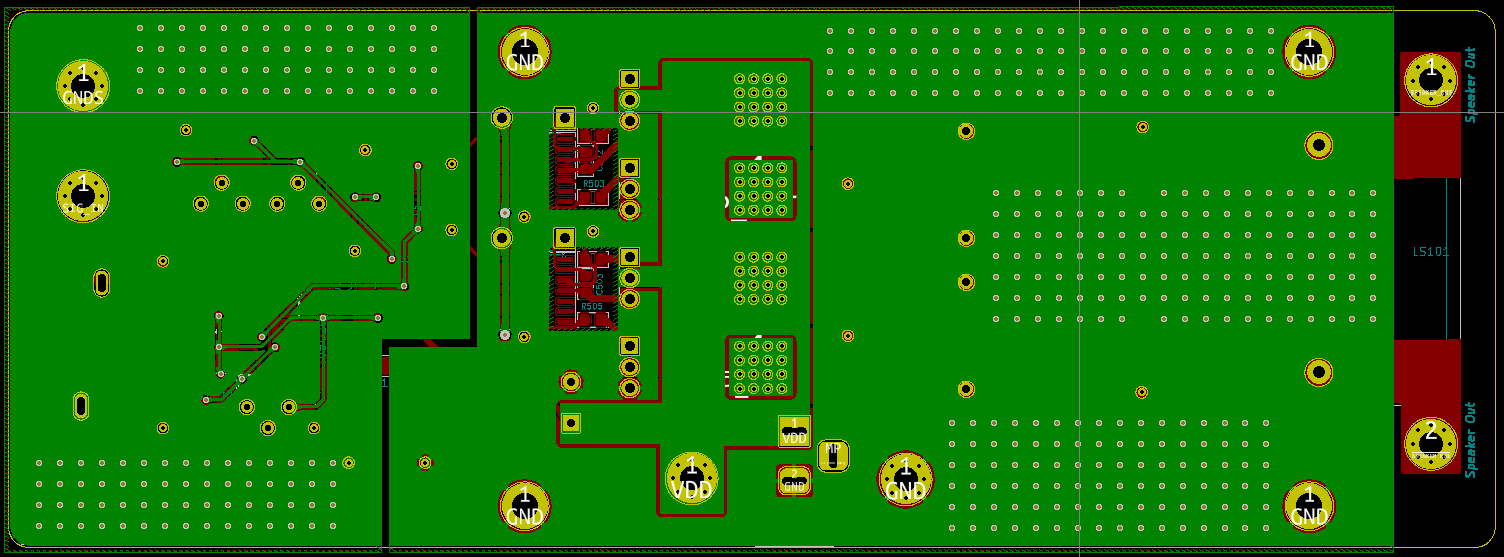
\includegraphics[width=\columnwidth]{pcb/bottom_layer.png}
        \subcaption{PCB bottom layer copper pours}
    \end{subfigure}
    \caption{Design PCB layouts}
\end{figure}


\begin{figure}[h!]
    \centering
    \begin{subfigure}{0.52\textwidth}
        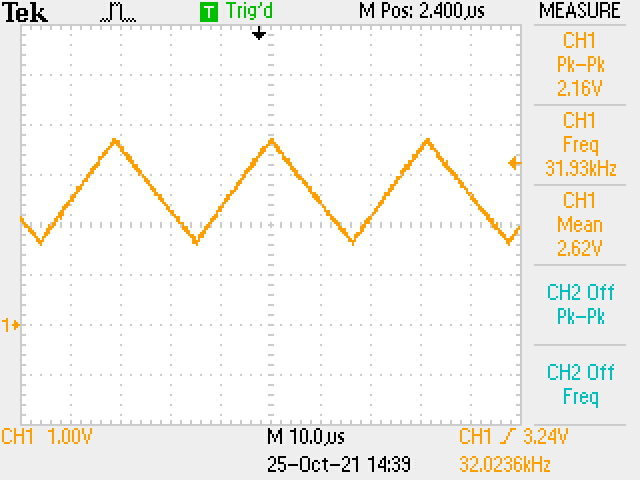
\includegraphics[width=\columnwidth]{spwm/triangle_wave_32kHz.JPG}
        \subcaption{Generated sampling triangle wave}
    \end{subfigure}
    \begin{subfigure}{0.48\textwidth}
        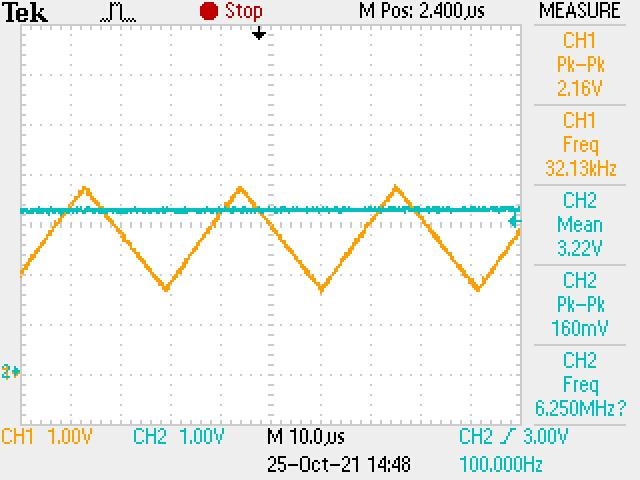
\includegraphics[width=\columnwidth]{spwm/input_sampling_1.JPG}
        \subcaption{Triangle wave sampling input signal}
    \end{subfigure}
    \begin{subfigure}{0.48\textwidth}
        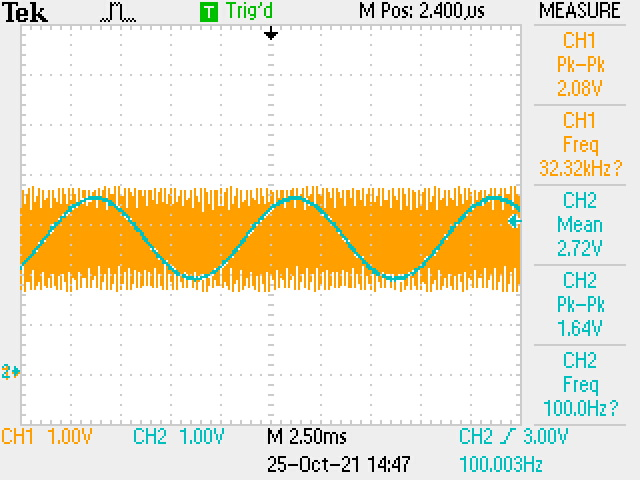
\includegraphics[width=\columnwidth]{spwm/input_sampling_0.JPG}
        \subcaption{Triangle wave sampling envelop of input signal}
    \end{subfigure}
    \caption{}
\end{figure}

\begin{figure}[h!]
    \centering
    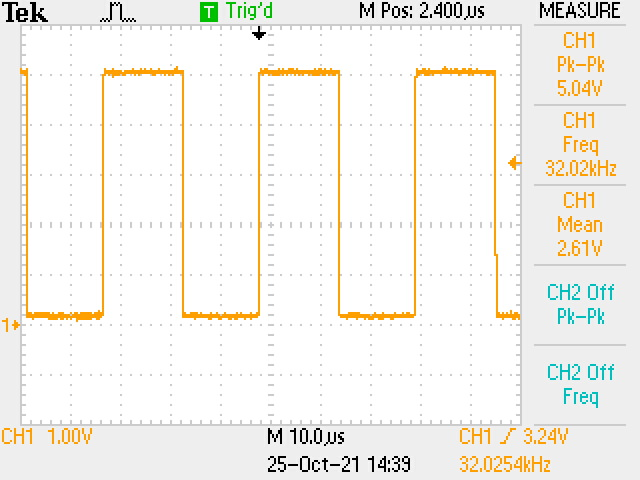
\includegraphics[width=0.65\textwidth]{spwm/spwm_no_input.JPG}
    \caption{Amplifier output bode plot}
\end{figure}


\section{Results}

Here I would expect to see the results of the whole amp, for example: an output wave, analysis of the efficiency, discuss maximum power output (which may be frequency dependent), and THD.


\begin{figure}[h!]
    \centering
    \begin{subfigure}{0.3\textwidth}
        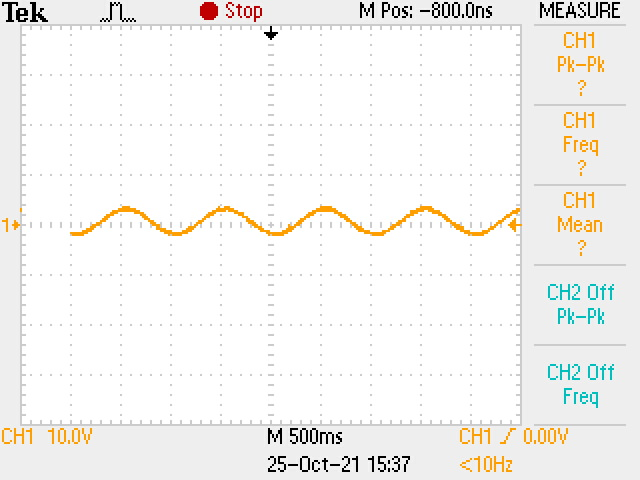
\includegraphics[width=\columnwidth]{power_output/filter_output_1Hz.JPG}
        \subcaption{1Hz}
    \end{subfigure}
    \begin{subfigure}{0.3\textwidth}
        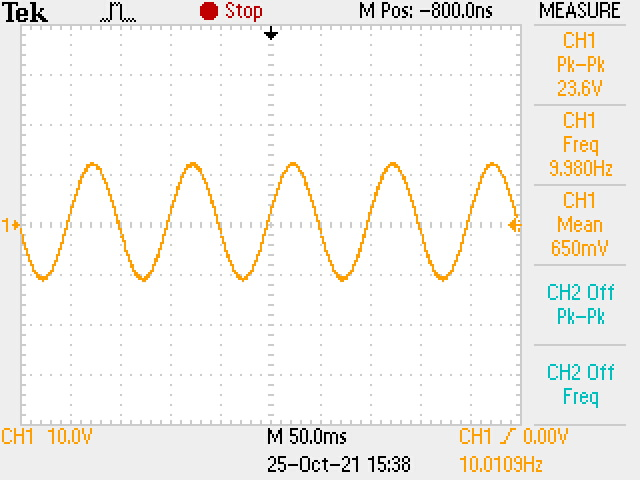
\includegraphics[width=\columnwidth]{power_output/filter_output_10Hz.JPG}
        \subcaption{10Hz}
    \end{subfigure}
    \begin{subfigure}{0.3\textwidth}
        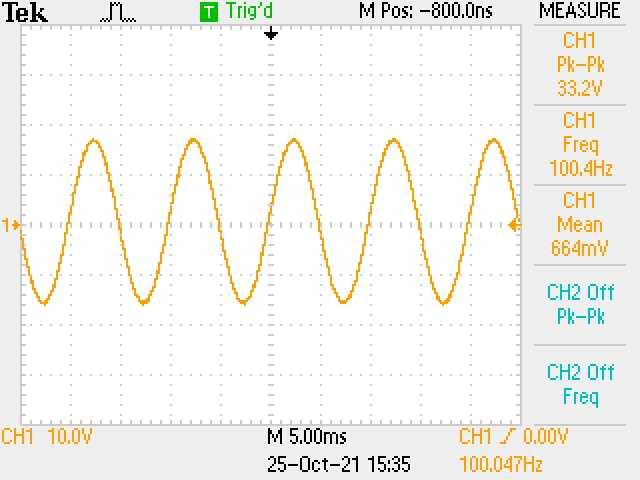
\includegraphics[width=\columnwidth]{power_output/filter_output_100Hz.JPG}
        \subcaption{100Hz}
    \end{subfigure}
    \begin{subfigure}{0.3\textwidth}
        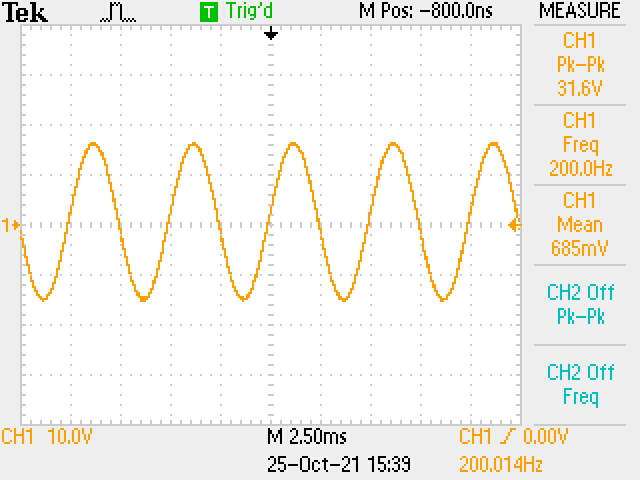
\includegraphics[width=\columnwidth]{power_output/filter_output_200Hz.JPG}
        \subcaption{200Hz}
    \end{subfigure}
    \begin{subfigure}{0.3\textwidth}
        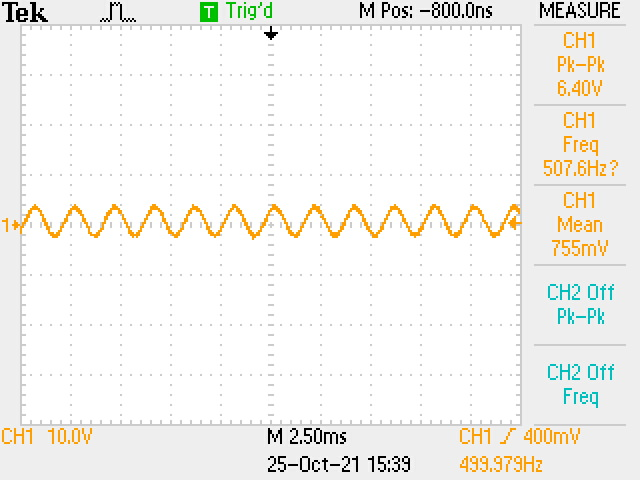
\includegraphics[width=\columnwidth]{power_output/filter_output_500Hz.JPG}
        \subcaption{500Hz}
    \end{subfigure}
    \begin{subfigure}{0.3\textwidth}
        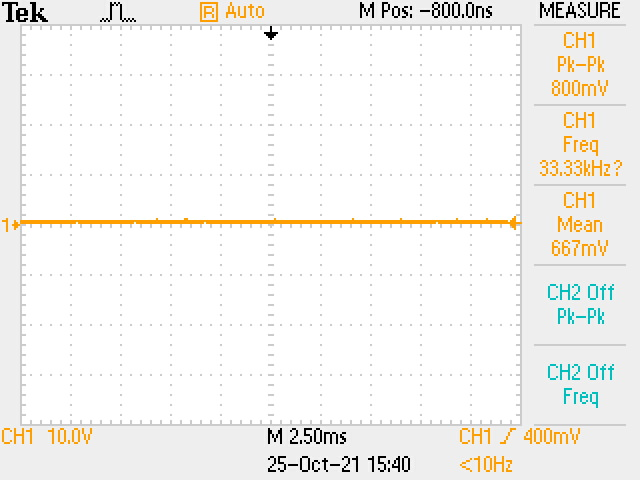
\includegraphics[width=\columnwidth]{power_output/filter_output_2kHz.JPG}
        \subcaption{2kHz}
    \end{subfigure}
    \caption{Amplifier output to varying frequency input signal}
\end{figure}


\begin{figure}[h!]
    \centering
    \frame{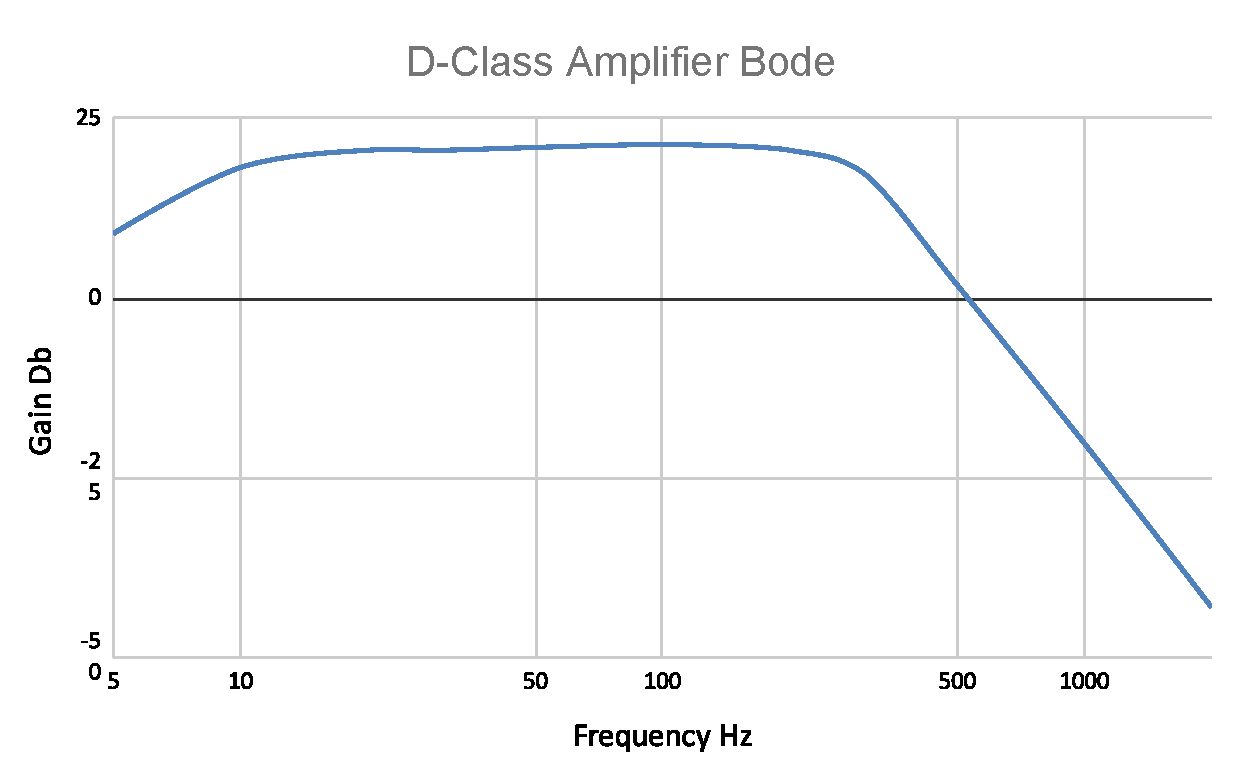
\includegraphics[width=0.85\textwidth]{power_output/amplifier_bode.pdf}}
    \caption{Amplifier output bode plot}
\end{figure}


\begin{figure}[h!]
    \centering
    \frame{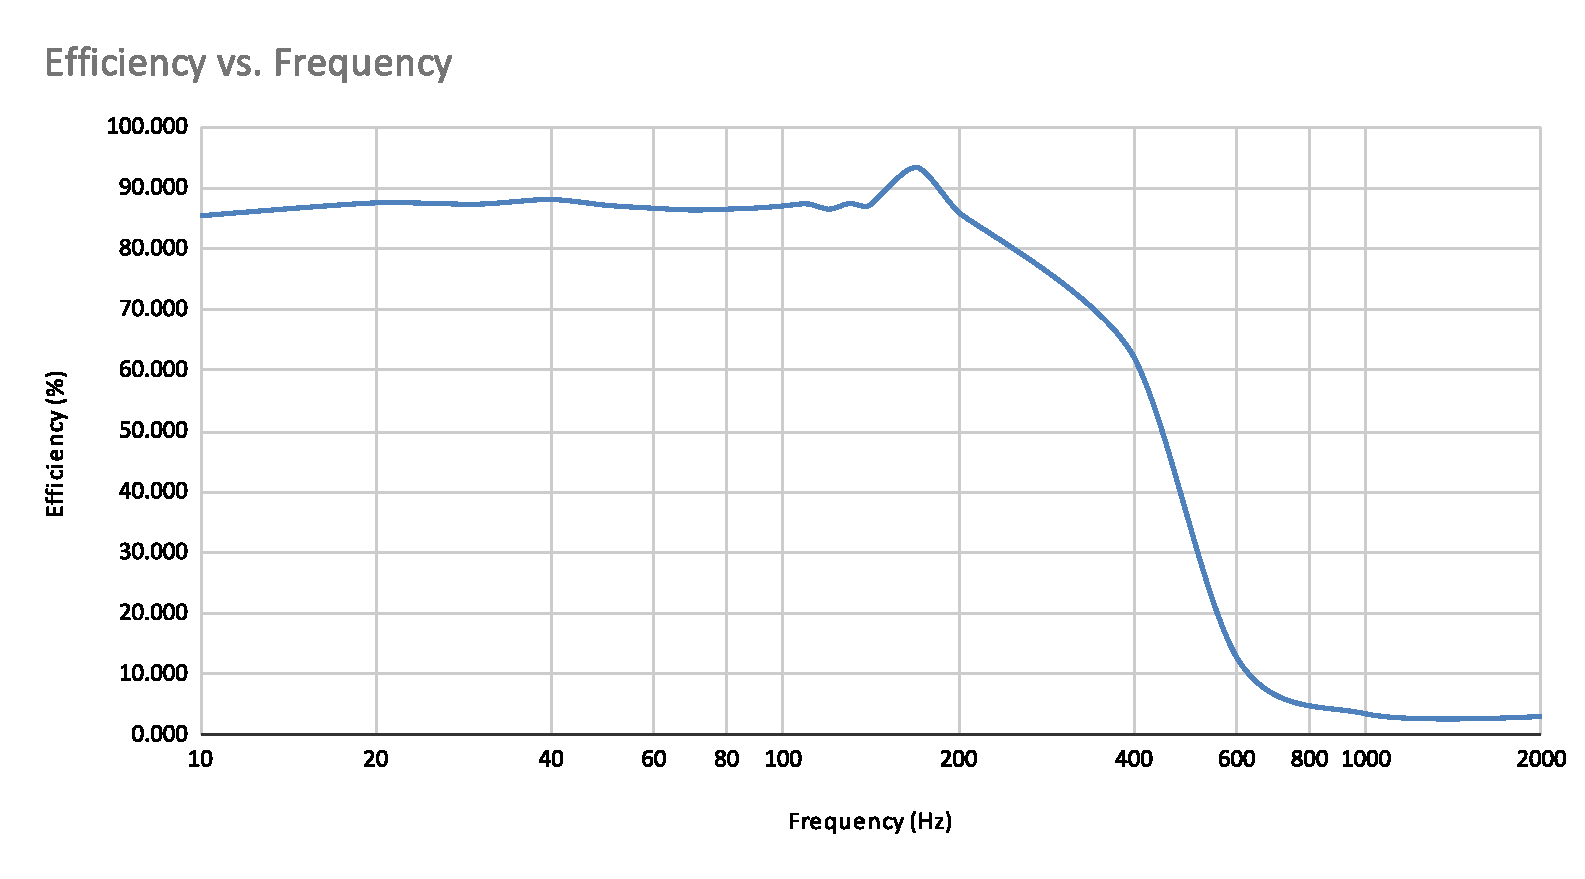
\includegraphics[width=0.85\textwidth]{power_output/Efficiency_vs._Frequency.pdf}}
    \caption{Amplifier output efficiency vs frequency}
\end{figure}


\begin{table}[h!]
    \centering
    \begin{tabular}{l|l}
    \rowcolor[HTML]{E0E0E0} 
    \textbf{Frequency (Hz)} & \textbf{THD (\%)} \\ \hline
    30                 & 1.8               \\
    50                 & 2.2               \\
    100                & 3.2               \\
    200                & 3.3               \\
    300                & 3.5               \\
    500                & 3.2              
    \end{tabular}
    \caption{Output total harmonic distortion across frequency}
    \label{T:THD}
\end{table}

\section{Conclusions}

What worked, didn’t work? How would you change your approach? Any interesting insights?

\clearpage
\section*{Appendix}
\subsection*{Input Filter}
\begin{figure}[h!]
  \centering
  \begin{subfigure}{0.3\textwidth}
    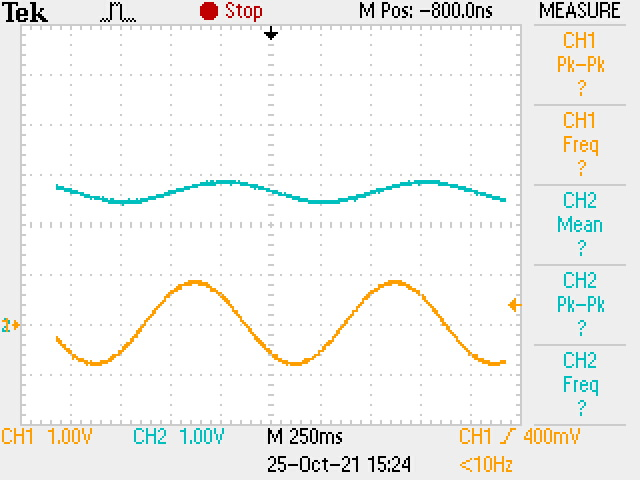
\includegraphics[width=\columnwidth]{input_filter/input_1Hz.JPG}
    \subcaption{1Hz}
  \end{subfigure}
  \begin{subfigure}{0.3\textwidth}
    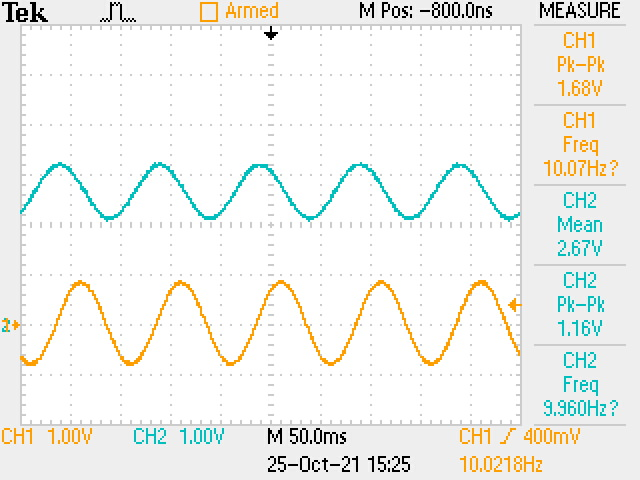
\includegraphics[width=\columnwidth]{input_filter/input_10Hz.JPG}
    \subcaption{10Hz}
  \end{subfigure}
  \begin{subfigure}{0.3\textwidth}
    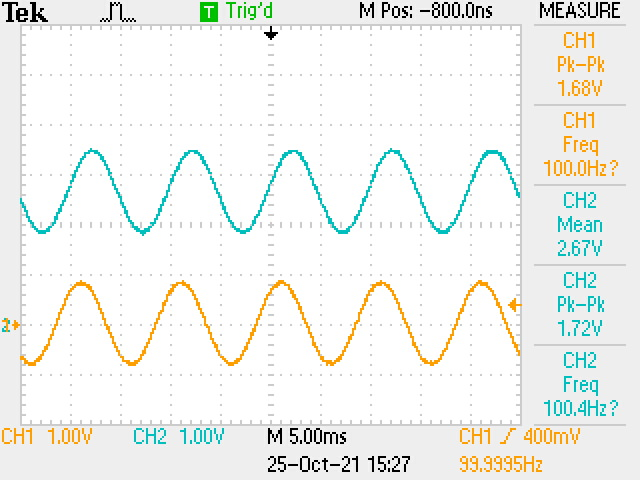
\includegraphics[width=\columnwidth]{input_filter/input_100Hz.JPG}
    \subcaption{100Hz}
  \end{subfigure}
  \begin{subfigure}{0.3\textwidth}
    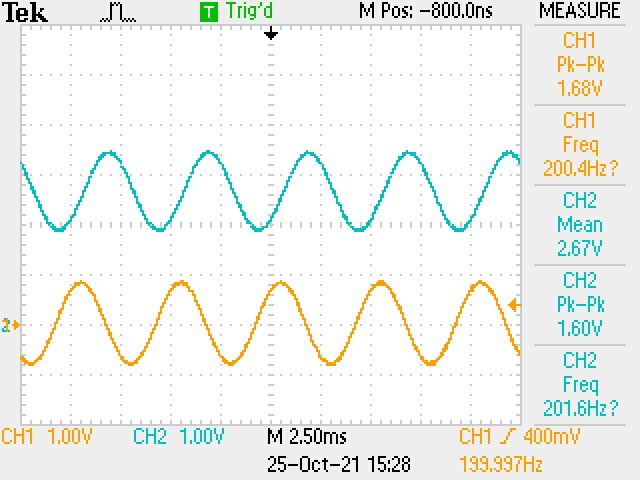
\includegraphics[width=\columnwidth]{input_filter/input_200Hz.JPG}
    \subcaption{200Hz}
  \end{subfigure}
  \begin{subfigure}{0.3\textwidth}
    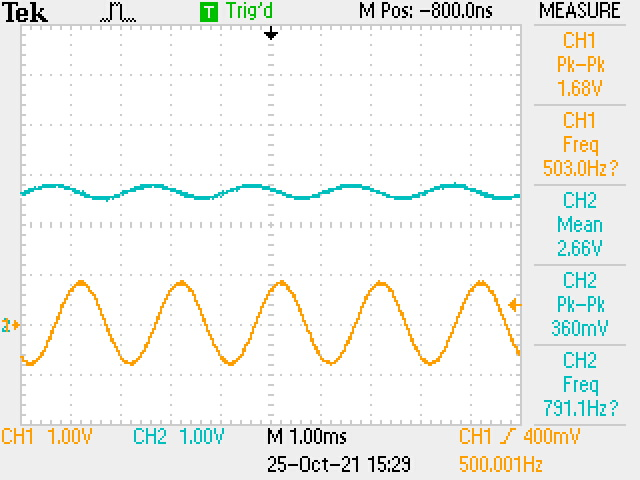
\includegraphics[width=\columnwidth]{input_filter/input_500Hz.JPG}
    \subcaption{500Hz}
  \end{subfigure}
  \begin{subfigure}{0.3\textwidth}
    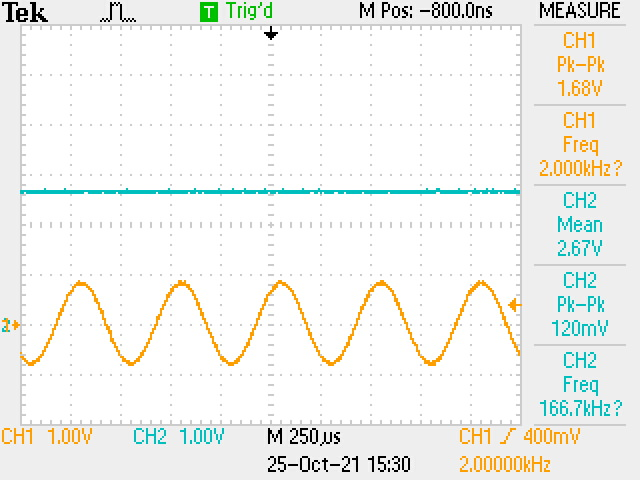
\includegraphics[width=\columnwidth]{input_filter/input_2kHz.JPG}
    \subcaption{2kHz}
  \end{subfigure}
  \caption{Input filter operation across frequencies, input signal (yellow) vs filter output (blue)}
\end{figure}


\end{document}